\graphicspath{{chapters/19/images/}}
\chapter{Rare events}

\section{Introduction}
Many observed transitions observed in biology could be considered rare events in the time scales of all atoms simulations.
This is because many processes require time-scales of seconds.

	\subsection{Rough free energy surfaces}
	The problem is that we have to deal with rough free energy surface with lots of local minima.
	Even in the case of \ref{fig:rough-free-energy} there are $4$ local minima, which is exponential for proteins.

	\begin{figure}[H]
		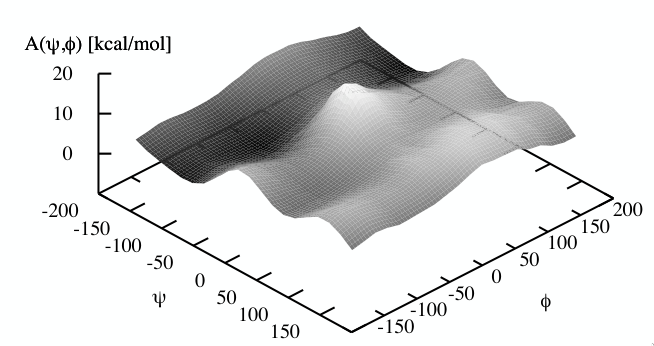
\includegraphics[width=\textwidth]{rough-free-energy-surfaces}
		\caption{Rough free energy surfaces}
		\label{fig:rough-free-energy-surfaces}
	\end{figure}

	The problem of studying this transition is difficult.

	\subsection{Variables in rare events}
	Describing the free-energy surface is difficult because the energies surfaces is complex.

		\begin{itemize}
			\item Reaction coordinates: how to describe a transition between states.
			\item Order parameters: they describe the transition between one energy minimum from another.
			\item COLVARs: collective variables.
		\end{itemize}

\section{Reaction coordinates}
There might be several reaction coordinates and the first problem is how to choose them.
This is system dependent.
For example considering dissociation reactions $AB\rightarrow A+B$ a good reaction coordinate could be the distance between the centre of mass of the atoms $r = |\vec{r}_B-\vec{r}_A|$.
Considering a protein, describing the transition from folded to unfolded one global measure is the radius of gyration:

$$R_G = \sqrt{\frac{1}{N_b}\sum\limits_{i=1}^{N_b}\biggl(\vec{r}_i-\frac{1}{N_b}\sum\limits_{j=1}^{N_b}\vec{r}_j\biggr)^2}$$

This gives a measure of how compact a protein is.
This is a good measure of foldedness in case of globular proteins, but this is not true for all proteins.
Another example is considering the number of hydrogen bonds between two elements of length $d_0$ between $n_O$ oxygens and $n_H$ hydrogens a good measure is:

$$N_H = \sum\limits_{i=1}^{n_O}\sum\limits_{j=1}^{n_H}\frac{1-\biggl[\frac{\vec{r}_i-\vec{r}_j}{d_0}\biggr]^6}{1-\biggl[\frac{\vec{r}_i-\vec{r}_j}{d_0}\biggr]^{12}}$$

So the objective is to obtain a single coordinate from the Cartesian coordinates so to understand the process that is happening.
After having obtained the reaction coordinates the aim is to obtain the probability distribution function of a subset of $n$ reaction coordinates of interest $q_\alpha= f_\alpha(\vec{r}_1, \dots, \vec{r}_N)$ with $\alpha = 1, \dots, n$ which will not be in general factorized and can be written as:

$$P(s_1, \dots, s_n) = \frac{C_N}{Q(N, V, T)}\int d^N\vec{p}d^B\vec{r}e^{-\beta\mathcal{H}(\vec{r}, \vec{p})}\prod\limits_{\alpha=1}^n\delta(f_\alpha(\vec{r}_1, \dots, \vec{r}_N)-s_\alpha)$$
For the canonical ensemble.
Once the probability is obtained the free energy hypersurface can be obtained directly:

$$A(s_1, \dots, s_n) = -fT\ln P(s_1, \dots, s_n)$$

If the right reaction coordinates are not chosen then free energy profiles might not be describing the system correctly.
To judge the quality of the chosen reaction coordinates is the committor distribution, an extremely expensive process but that can be worthwhile.

	\subsection{Blue moon ensemble}
	One method to obtain a rare events is the blue moon ensemble.
	When choosing a reaction coordinate the objective is to force a transition between states.
	The idea behind the blue moon ensemble is that considering for semplicity a single reaction coordinate $q_1 = f_1(\vec{r}_1, \dots, \vec{r}_N)$, its probability distribution is:

	$$P(s) = \frac{C_N}{Q(N, V, T)}\int d^N\vec{p}d^N\vec{r}e^{-\beta\mathcal{H}(\vec{r}, \vec{p})}\delta(f_1(\vec{r}_1, \dots, \vec{r}_N)-s)$$

	And the free energy profile:

	$$A(s) = -kT\ln P(s)$$

	Now a holonomic constraint is introduced $\sigma(\vec{r}_1, \dots, \vec{r}_N) = f_1(\vec{r}_1, \dots, \vec{r}_N)-s$.
	Then the sampling happens at that given value.
	So that the reaction coordinates assume a given set of values.
	Use this constraint to drive the reaction coordinate from an initial value $s^{(i)}$ to a final value $s^{(f)}$.
	The blue moon ensemble yields $\frac{dA}{ds} = -\frac{kT}{P(s)}\frac{dP}{ds}$.
	From this quantity then the free energy at any value of reaction coordinate $q$ can be reconstructed knowing the initial value.
	The free energy difference can be also computed:

	$$A(q) = A(s^{(i)}) + \int_{s^{(i)}}^q\frac{dA}{ds}ds\qquad \Delta A = \int_{s^{(i)}}^{s^{(f)}}\frac{dA}{ds}ds$$

	The probability distribution for the reaction coordinate $s$ is given by:

	$$P(s) = \frac{C_N}{Q(N, V, T)}\int d^N\vec{p}d^N\vec{r}e^{-\beta\mathcal{H}(\vec{r}, \vec{p})}\delta(f_1(\vec{r}_1, \dots, \vec{r}_N)-s) = \langle\delta(f_1(\vec{r}_1, \dots, \vec{r}_N)-s)\rangle$$

	So now the quantity obtained from the simulation:

	$$\frac{1}{P(s)}\frac{dP}{ds} = \frac{C_N}{Q(N, V, T)}\frac{\int d^N\vec{p}d^N\vec{r}e^{-\beta\mathcal{H}(\vec{r}, \vec{p})}\frac{\partial\delta(f_1(\vec{r})-s)}{\partial s}}{\langle\delta(f_1(\vec{r})-s)\rangle}$$

	Introduce $3N$ generalized coordinates $q_\alpha = f_\alpha(\vec{r}_1, \dots, \vec{r}_N)$ so that $q_1$ is the reaction coordinate of interest and their conjugate momenta $p_\alpha$,
	The transformation is canonical, hence the Jacobian is one: $d^N\vec{p}d^N\vec{r} = d^{3N}pd^{3N}q$, so the quantity is:

	$$\frac{1}{P(s)}\frac{dP}{ds} = \frac{C_N}{Q(N, V, T)}\frac{\int d^{3N}pd^{3N}qe^{-\beta\tilde{\mathcal{H}}(q, p)}\frac{\partial\delta(q_1-s)}{\partial s}}{\langle\delta(q-s)\rangle}$$

	However $\frac{\partial}{\partial s}\delta(q_1-s) = -\frac{\partial}{\partial q_1}\delta(q_1-s)$ substituting in the integral and integrating by parts:

	\begin{align*}
		\frac{1}{P(s)}\frac{dP}{ds} &=-\frac{\beta C_N}{Q(N, V, T)}\frac{\int d^{3N}pd^{3n}q\frac{\partial\tilde{\mathcal{H}}}{\partial q_1}e^{-\beta\tilde{\mathcal{H}}(q, p)}\delta(q_1-s)}{\langle\delta(q_1-s)\rangle} = \\
																&= -\frac{\beta}{\langle\delta(q_1-s)\rangle}\biggl\langle\frac{\partial\tilde{\mathcal{H}}}{\partial q_1}\delta(q_1-s)\biggr\rangle \equiv -\beta\biggl\langle\frac{\partial\tilde{\mathcal{H}}}{\partial q_1}\biggr\rangle^{cond}
	\end{align*}

	In this way everything can be expressed in term of the conditional average subject to the condition that $q_1=s$.
	So the simulation is run and the average value of the quantity is taken thanks to the holonomic constraint.
	This is measured with different initial values so that in the end the free energy as a function of the reaction coordinate:

	$$A(q) = A(s^{(i)}) + \int_{s^{(i)}}^q\biggl\langle\frac{\partial\tilde{\mathcal{H}}}{\partial q_1}\biggr\rangle^{cond}_sds$$

	\subsection{Umbrella sampling}
	Umbrella sampling substitutes the rigid holonomic contraints of blue moon sampling with a more flexible harmonic restraint.
	So an extra potential or bias potential is introduced such that the reaction coordinates are constraint to be close to the value $s_k$:

	$$W_k(f_1(\vec{r}_1, \dots, \vec{r}_N), s_k) = \frac{1}{k}[f_1(\vec{r}_1, \dots, \vec{r}_N)-s_k]^2$$

	The probability distribution for $s$ is biased to be close to $s_k$.
	The biased probability distributions obtained will be:

	$$P(s, s^{(k)}), k= 1, \dots, n,\qquad s^{(1)}=s^{(i)}, s^{(n)}=s^{(f)}$$

	Now from this is obtained a collection of biased probability distribution, one for each value of $k$.
	This probability distribution should be used to reconstruct the real one.
	To do so the weighted histogram analysis method.

	\subsection{WHAM}
	The weighted histogram analysis method is used to obtain from the collection of biased probability distribution obtained from umbrella sampling the real one.
	So for each of the $k$ biased probability distributions generated by umbrella sampling:

	$$\tilde{P}(q, s^{(k)}) = e^{\beta A_k}\int d^N\vec{r}e^{-\beta U(\vec{r})}e^{-\beta W_k(f_1(\vec{r}), s^{(k)})}\delta(f_1(\vec{r})-q)$$

	Where $e^{\beta A_k}$ is the normalization factor and $A_k$ is the free energy associated with the biasing potential apart from constants so that:

	$$e^{-\beta A_k} = \int d^N\vec{r}e^{-\beta U(\vec{r})}e^{-\beta W_k(f_1(\vec{r}), s^{(k)})}=e^{-\beta A_0}\biggl\langle e^{-\beta W_k(f_1(\vec{r}), s^{(k)})}\biggr\rangle$$

	The average is taken with respect to the unbiased potential:

	$$e^{-\beta A_0} = \int d^N\vec{r}e^{-\beta U(\vec{r})}$$

	To unbiased the probability distributions the Boltzmann factor is introduced:

	$$P_k(q) = e^{-\beta(A_k-A_0)\beta W_k(q, s^{(k)})}\tilde{P}(q, s^{(k)})$$

	Now a collection of $n$ unbiased probability distribution is obtained that describe a single region of the possible values of the reaction coordinates.
	To reconstruct the full probability distribution the objective is to combine them into a single one.
	To do that these distribution are combined with weights $C_k$ such that $\sum\limits_{k=1}^n C_k=1$, so the total probability distribution is:

	$$P(q) = \sum\limits_{k=1}^n C_k(q)P_k(q) = \sum\limits_{k=1}^nC_k(q)e^{-\beta(A_k-A_0)}e^{\beta W_k(q, s^{(k)})}\tilde{P}(q, s^{(k)})$$

	Now the values of $C_k$ have to be obtained using a criterion, to the statistical error in the distribution generated by the WHAM procedure is minimized.
	To obtain the biased probability distribution let $\tilde{H}_k(q)$ be the biased histogram obtained from each molecular dynamics or Monte Carlo simulation.
	So the system will be in that position from a given number of frame.
	The estimate for the biased distributions is:

	$$\tilde{P}(q, s^{(k)}) \approx\frac{1}{n_k\Delta q}\tilde{H}_k(q)$$

	Where:

	\begin{multicols}{2}
		\begin{itemize}
			\item $n_k$ is the number of frames in an umbrella window.
			\item $\Delta q$ takes into account that the possible value of the reaction coordinate are in bins.
		\end{itemize}
	\end{multicols}

	The statistical error for the umbrella window is

	$$\tilde{\sigma}^2_k = \frac{\epsilon_k(q)\tilde{H}_k(q)}{n_k\Delta q}$$

	Where $\epsilon_k$ is a given factor.
	This is because since there are a number of occurrences of these stochastic process the number of occurrences is a Poisson process.
	The error in $P_k(q)$ (the unbiased probability distribution) is given by applying the square of the unbiasing  factor:

	$$\sigma_k^2 = e^{-2\beta(A_k-A_0)}e^{2\beta W_k(q, s^{(k)})}\tilde{\sigma}_k^2$$

	So the total error will be:

	$$\sigma^2 = \sum\limits_{k=1}^nC_k^2(q)\sigma_k^2$$

	To minimize the total statistical error considering the condition that the sum over the $C_k$ is equal to $1$.
	To do so Lagrange multipliers are used.
	Then the function to minimize is:

	$$\Sigma^2=\sum\limits_{k=1}^nC_k^2(q)e^{-2\beta (A_k-A_0)}e^{w\beta W_k(q, s^{(k)})}\frac{\epsilon_k(q)\tilde{H}_k(q)}{n_k\Delta q}-\lambda\biggl(\sum\limits_{k=1}^nC_k(q)-1\biggr)$$

	The unknowns are $C_k$ and $\lambda$, so now to minimize:

	$$\frac{\partial\Sigma^2}{\partial C_k(q)} = 0\Rightarrow C_k(q) = \frac{\lambda n_k\Delta q}{2\epsilon_k(q)\tilde{H}_k(q)e^{-2\beta(A_k-A_0)}e^{2\beta W_k(q, s^{(k)})}}$$

	So all the $C_k$ depends on $\lambda$.
	$\lambda$ is unknown and to determine it the normalization condition is used:

	$$\lambda = \frac{1}{\sum\limits_{k=1}^n\frac{n_k\Delta q}{2\epsilon_k(q)\tilde{H}_k(q)e^{-2\beta(A_k-A_0)}e^{2\beta W_k(q, s^{(k)})}}}$$

	Now the solution for $C_k$ is obtained:

	$$C_k(q) =\frac{n_kl\bigl[\epsilon_k(q)\tilde{H}_k(q)e^{-2\beta(A_k-A_0)}e^{2\beta W_k(q, s^{(k)})}\bigr]}{\sum\limits_{j=1}^n n_jl\bigl[\epsilon_j(q)\tilde{H}_j(q)e^{-2\beta(A_j-A_0)}e^{2\beta W_k(q, s^{(j)})}\bigr]}$$

	Now considering the following simplifying assumption that they need to be checked in the system:

	\begin{multicols}{2}
		\begin{itemize}
			\item $\epsilon_k(q)$ is the same for all umbrella windows.
				This does not imply that all the umbrella windows are of the same size, but that the quality of sampling is the same for all of them.
			\item $\tilde{H}_k(q)\propto e^{\beta(A_k-A_0)}e^{-\beta W_k(q, s^{(k)})}P(q)$.
				The histogram of the probability distribution is proportional to the real distribution biased by the two factors.
		\end{itemize}
	\end{multicols}

	Assuming these $C_k$ can be simplified into:

	$$C_k(q) = \frac{n_ke^{\beta A_k}e^{-\beta W_k(q, s^{(k)})}}{\sum\limits_{j=1}^nn_je^{\beta A_j}e^{-\beta W_j(q, s^{(j)})}}$$

	Using this formula the full probability distribution will be:

	$$P(q) = \sum\limits_{k=1}^nC_k(q)P_k(q) = \frac{\sum\limits_{k=1}^nn_k\tilde{P}(q, s^{(k)})}{\sum\limits_{k=1}^nn_ke^{\beta(A_k-A_0)}e^{-\beta W_k(q, s^{(k)})}}$$

	However:

	$$e^{\beta(A_k-A_0)} = \int dq P(q)e^{-\beta W_k(q, s^{(k)})}$$

	These two equations are self consistent because one depends on the other, so the algorithm starts with a guess for $A_k$ and iterates until convergence.

	\subsection{Wang-Landau sampling}
	In the Wang-Landau approach the density of states were the objective with a Monte Carlo simulation.
	So after devising some moves they where accepted with probability:

	$$A(\vec{r}_2|\vec{r}_1) = \min\biggl[1, \frac{\Omega(E_1)}{\Omega(E_2)}]\biggr]$$

	With scaling factor $f$ to scale the density of state each time one state was visited.
	The same can be Extended to reaction coordinates: generate a function $g(s)$ that approaches the probability distribution $P(s)$.
	Start $g(s)=1$ and $h(s) = \ln g(s) = 0$ everywhere, then the same procedure is performed: a move is generated and accepted with:

	$$A(\vec{r}_2|\vec{r}_1) = \min\biggl[1, \frac{e^{-\beta U(\vec{r}_2)}}{e^{-\beta U(\vec{r}_1)}}\frac{g(s_1)}{g(s_2)}\biggr] = \min\biggl[1, \frac{e^{-\beta U(\vec{r}_2)}}{e^{-\beta U(\vec{r}_1)}}\frac{e^{-h(s_1)}}{e^{-h(s_2)}}\biggr]$$

	Every time a new value of $s$ is visited $h$ is update by adding a factor $\alpha$:

	$$h(s_2) \rightarrow h(s_2) + \alpha \Leftrightarrow g(s_2)\rightarrow fg(s_2)\qquad \alpha = \ln f$$

	Iterate until the histogram $H(s)$ becomes flat, then reduce $f$ and repeat until convergence.
	When convergence is reached $P$ is obtained.
	Its efficiency and accuracy depends on the choice of reaction coordinates.
